\hypertarget{symetric-cryptography}{%
\section{Symetric Cryptography}\label{symetric-cryptography}}

\textbf{Definitions:} \\
X: set of plaintexts \\
Y: set of ciphertexts \\
Z: set of keys \\
Encryption: $E_z: X \xrightarrow{} Y$ with $z \in Z$ \\
Decryption: $D_z: Y \xrightarrow{} X$ with $z \in Z$\\

\hypertarget{symetrische-kryptographie}{%
\subsection{Symetrische Kryptographie}\label{symetrische-kryptographie}}

\begin{tcolorbox}[colback=red!5!white,colframe=red!75!black]
Symmetrisch bedeutet, dass ich für die VERschlüsselung und die ENTschlüsselung, denselben Schlüssel benutze. 
\end{tcolorbox}

\hypertarget{attacken}{%
\subsection{Attacken}\label{attacken}}

\begin{tcolorbox}[colback=red!5!white,colframe=red!75!black]
Wir nehmen immer an, dass der Angreiffer den Algorithmus bzw. das Verfahren kennt. 
Die Sicherheit beruht alleine auf der Geheimhaltung des Schlüssels und nicht auf der Geheimhaltung des Verfahrens.
\textbf{-> Kerckhoff's principle}
\end{tcolorbox}

\hypertarget{szenarien-fuxfcr-den-angreiffer}{%
\subsubsection{Szenarien für den Angreiffer}\label{szenarien-fuxfcr-den-angreiffer}}

\begin{itemize}
\tightlist
\item
  \textbf{Ciphertext-only}\\
  Der Angreiffer kennt nur den Verschlüsselten Text. Ist eher schwierig.
\item
  \textbf{Known Plaintext}\\
  Der Angreiffer kennt zumindest ein Teil des Klartextes. Davon kann man
  heute in aller Regel ausgehen.
\item
  \textbf{Chosen Plaintext}\\
  Ich erbeute eine Verschlüsselungsmaschine und kann beliebige
  Textbausteine verschlüsseln und probieren.
\end{itemize}

\hypertarget{blockverschluxfcsselung}{%
\subsection{Blockverschlüsselung (Block Cipher)}\label{blockverschluxfcsselung}}

\begin{itemize}
\tightlist
\item
  Wir haben ein Alphabet mit Symbolen
\item
  Die Blocklänge n ist fixiert
\end{itemize}

Es kommen immer n Klartext-Symbole rein und es kommen immer n Geheimtext-Symbole raus (unter den folgenden Bedingunen). Über die Länge des Schlüssels gibt es hier keine Aussage.

\hypertarget{bedingungen-blockverschlüsselung}{%
\subsubsection{Bedingungen zur Blockverschlüsselung}\label{bedingungen-blockverschlüsselung}}

\begin{itemize}
\tightlist
\item
  \textbf{Injective}: Wenn zwei Geheimtexte gleich sind, müssen auch die
  Klartexte gleich sein. Das heisst ein Geheimtext darf nur auf ein
  eindeutiger Klartext abgebildet werden können.
\item
  \textbf{Surjective}: Für jeden Geheimtext gibt es einen Klartext. Es
  gibt keinen Geheimtext, der nicht auf einen Klartext abgebildet werden
  kann.
\end{itemize}

\begin{tcolorbox}[colback=red!5!white,colframe=red!75!black]
Die obigen Bedingunen ergeben dann -> Bijective Self-Mapping
\end{tcolorbox}

\hypertarget{lineare-funktionen}{%
\subsubsection{Lineare Funktionen}\label{lineare-funktionen}}

$Z_m$ bedeutet alle ganze Zahlen von 0 bis m-1.

\begin{figure}[H]
\centering
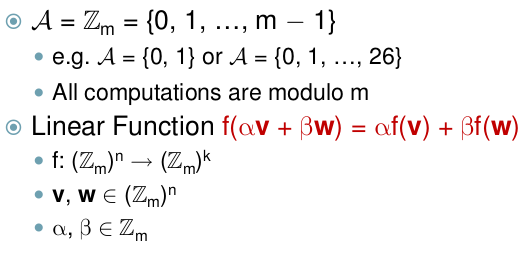
\includegraphics[width=0.5\textwidth]{figures/linearFunctions.png}
\caption{Linear Functions}
\end{figure}

\hypertarget{affine-map}{%
\subsubsection{Affine Map}\label{affine-map}}

\textbf{Affine bedeutet linear plus einen konstanten Vektor.}

\begin{figure}[H]
\centering
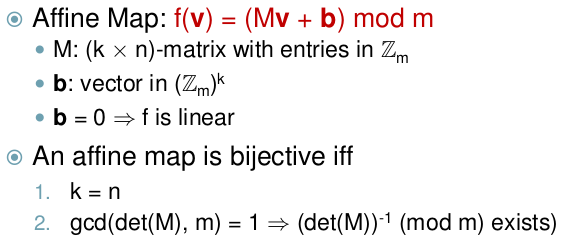
\includegraphics[width=0.65\textwidth]{figures/affineMap.png}
\caption{Affine Map}
\end{figure}

\hypertarget{vigenuxe8re-cipher}{%
\subsection{Vigenère Cipher}\label{vigenuxe8re-cipher}}

\textbf{Ist nicht sicher}. Durch Stochastischee Analyse kann man die Länge des
Geheimwortes ausfindig machen und den Geheimtext in Gruppen der
Geheimwort-Buchstaben einteilen. Wenn man zudem nur Teile des
Geheimwortes kennt, könnte man auf das ganze Geheimwort schliessen (Da
das Geheimwort auch eine Struktur oder Sinn hat).

\begin{figure}[H]
\centering
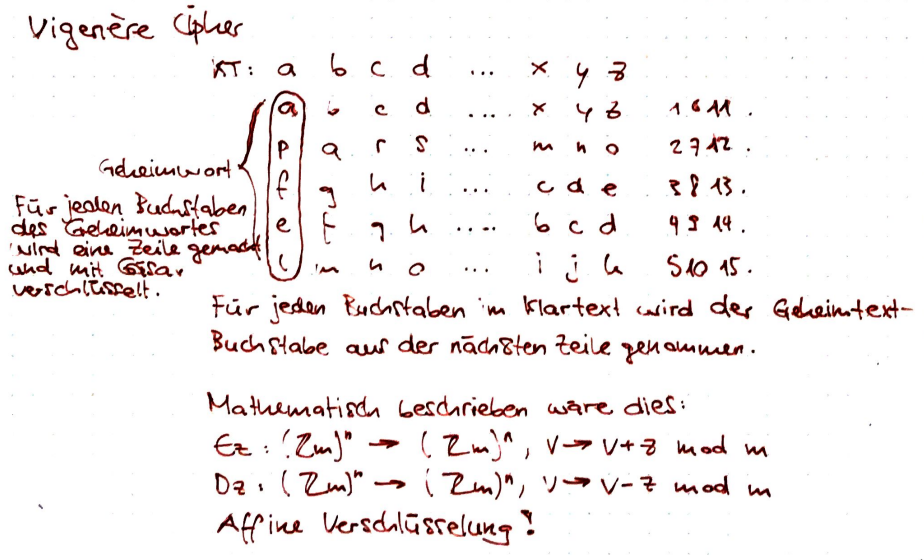
\includegraphics[width=0.5\textwidth]{figures/vigenereCipher.png}
\caption{Vigenere Cipher}
\end{figure}

\hypertarget{one-time-pad}{%
\subsection{One-time Pad}\label{one-time-pad}}

Wenn folgende Bedingungen zur Erweiterung von der Vigenère Cipher
erfüllt sind, ist die Verschlüsselung sicher: 
\begin{itemize}
    \item Das Schlüsselwort ist mindestens solange wie der grösste jemals zu verschlüsselnde Klartext.
    \item Das Schlüsselwort ist rein zufällig gewählt ohne Struktur oder Sinn
\end{itemize}

\begin{figure}[H]
\centering
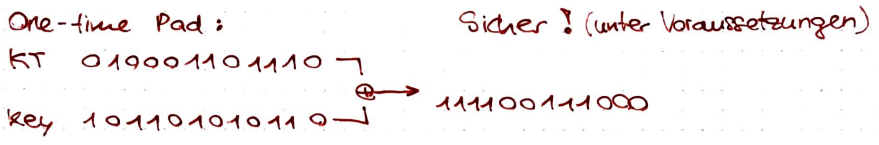
\includegraphics[width=1\textwidth]{figures/onetimePad.png}
\caption{One-time Pad}
\end{figure}

\hypertarget{hill-cipher}{%
\subsection{Hill Cipher}\label{hill-cipher}}

Als Schlüssel wird eine invertierbare nxn-Matrix gewählt. Wir brauchen also

\begin{figure}[H]
\centering
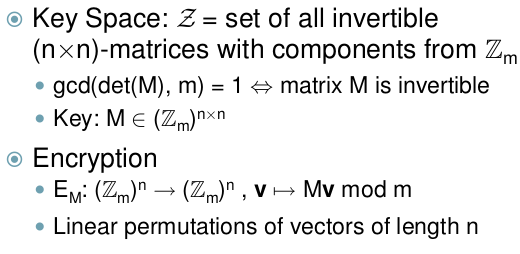
\includegraphics[width=0.6\textwidth]{figures/hillCipher.png}
\caption{Hill Cipher}
\end{figure}

\hypertarget{general-affine-cipher}{%
\subsection{General Affine Cipher}\label{general-affine-cipher}}

Zusätzlich zur Hill-Verschlüsselung wird noch ein konstanter Vektor b hinzugefügt. Nach der Verschlüsselung mit Hill wird der Geheimtext noch der konstante Vektor b addiert.

\begin{figure}[H]
\centering
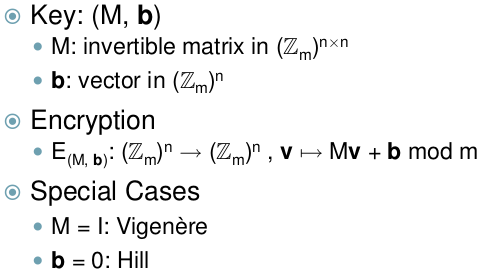
\includegraphics{figures/generalAffineCipher.png}
\caption{General Affine Cipher}
\end{figure}

\begin{tcolorbox}[colback=red!5!white,colframe=red!75!black]
    Jede Affine Verschlüsselung ist nicht sicher und damit knackbar.
\end{tcolorbox}

\hypertarget{confusion-diffusion}{%
\subsection{Confusion \& Diffusion}\label{confusion-diffusion}}

F = Mathematische Funktion zur Abbildung des Klartextes in Geheimtext

\textbf{Confusion}: Verwirrung des Gegners. - F muss mathematisch
komplex sein - Für ein gegebenes x und y darf nicht auf z geschlossen
werden - F darf nicht linear sein!

\textbf{Diffusion}: Jedes Ausgangsbit muss auf irgendeine Weise von
\textbf{JEDEM} Eingangsbit abhängig sein. Es darf nicht sein, dass die erste
Hälfte des Geheimtextes nur von der ersten Hälfte des Klartextes
abhängig ist. - Changing a single bit in the plaintext (or the key), on
the average 50\% of the ciphertext bits should change - Every ciphertext
bit should depend on every plaintext and every key bit
\newline
\newline
Diffusion erreicht man häufig, in dem man verschiedene Runden hat. Wie
z.B. beim Karten mischen, in welchem man das Mischeln wiederholt, um
eine bessere Diffusion zu erhalten.

\textit{\hl{Electronic Code Book kommt in Kapitel Block Modes}}

\clearpage